\section{Pattern Matching with Typed Holes}

Let us now return to languages with holes, considering how we can implement pattern matching while maintaining the maximal liveness invariant. Presently, all current systems only support holes in expressions or types, but not in binding constructs. Thus, when editing a pattern itself, intermediate states are not well-formed terms, and they can be given neither static nor dynamic meaning. To correct this, we must extend our notion of holes to also include \emph{pattern holes}. Analogously to expression holes, we include two variants: \emph{empty pattern holes} indicate a missing sub-term of a pattern, while \emph{non-empty pattern holes} surround patterns that may be ill-typed with regards to their location in a larger pattern. With this, we can indeed represent any intermediate pattern edit state, but the question remains of what static and dynamic semantics can be given to these pattern holes.

To express the semantics of a \li{match} expression with holes, it suffices to specify what it means for a single expression to match a single pattern. In order to ensure soundness with respect to filling holes at a later point in time, we must reason conservatively about all possible hole fillings. Concretely, consider the expression $1 :: \hehole{u} :: []$ matched against various patterns, where $\hehole{u}$ indicates an empty hole which we label with the id $u$. Regardless of how this hole is filled, the resulting expression will always be a non-empty list and thus will always match the pattern $hd :: tl$. Likewise, any hole filling of $1 :: \hehole{u} :: []$ cannot match any hole filling of the pattern $\heholep{w} :: []$, since the former will always have three elements while the latter only has one. As a result, we can soundly state that $1 :: \hehole{u} :: []$ \emph{must} match the pattern $hd :: tl$ but \emph{must not} match $\heholep{w} :: []$. 

Most interesting, however, is when different hole fillings give rise to different behavior. For example, consider matching $1 :: \hehole{u} :: []$ against the pattern $1 :: 2 :: \hehole{w}$. If $\hehole{u}$ is filled with $2$ and $\hehole{w}$ is filled with a variable or the empty list $[]$, then this match will succeed. However, the match will fail with any other hole filling, so without knowledge of the future contents of these holes, we cannot soundly reason about the result of this match. That is, we can only state that $1 :: \hehole{u} :: []$ \emph{indeterminately} matches $1 :: 2 :: \hehole{w}$: for some hole fillings it does, for others it does not.

\todo{The in-text expressions here might be better placed into some figure}

Thus, when we allow expression and pattern holes, we can no longer determinately say whether an expression matches a given pattern. What was once a binary decision (either $e$ matches $p$ or $e$ does not match $p$) is now a ternary decision: either $e$ must match $p$, $e$ must not match $p$, or $e$ indeterminately matches $p$ depending on how the various holes are filled. In this setting, the semantics of a \li{match} expression can act similarly to before, but evaluation must pause if the scrutinee indeterminately matches the pattern under consideration, waiting for the user to fill holes to continue.
Likewise, redundancy and exhaustiveness also become ternary decisions: a \li{match} expression may either be definitely exhaustive, definitely non-exhaustive, or indeterminate, and likewise for redundancy. We leave a more detailed discussion of these analyses to our full paper. 

With this, we have identified the main contributions our proposal will make. We seek to develop a calculus which formalizes the above discussion, allowing pattern matching with holes in both expressions and patterns. We will maintain maximal liveness by identifying when a match is indeterminate and when an expression can no longer be evaluated without further hole-filling, and we will develop a means to statically perform (possibly indeterminate) exhaustiveness and redundancy checking in this setting.

%\subsection{Exhaustiveness Checking with Pattern Holes}
%
%\begin{figure}
%	\centering
%	% Capture tallest image in box 3
%	\setbox3=\hbox{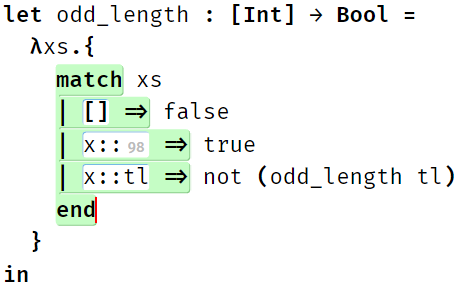
\includegraphics[scale=0.45]{imgs/exhaustive.png}}%
%	\subcaptionbox{Indeterminately Exhaustive\label{fig:may-exhaustive}}{
%		\raisebox{\dimexpr\ht3-\height}{
%			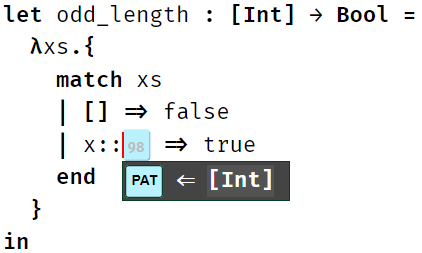
\includegraphics[scale=0.45,valign=t]{imgs/maybe_exhaustive.png}%
%			\vphantom{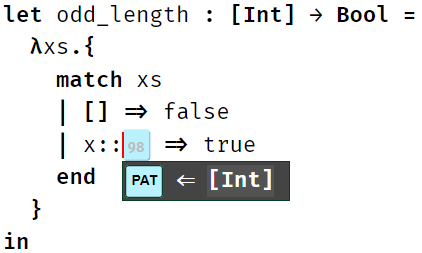
\includegraphics[scale=0.45,valign=t]{imgs/maybe_exhaustive.png}}
%		}
%	}
%	\hfil
%	\subcaptionbox{Necessarily Inexhaustive\label{fig:not-exhaustive}}{
%		\raisebox{\dimexpr\ht3-\height}{
%			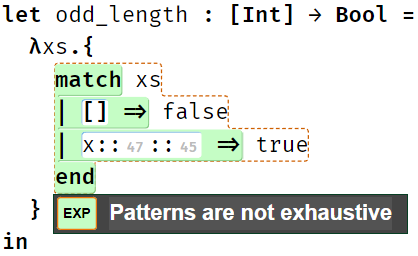
\includegraphics[scale=0.45,valign=t]{imgs/not_exhaustive.png}%
%			\vphantom{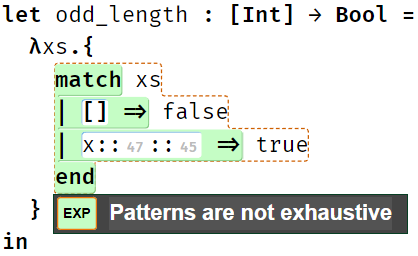
\includegraphics[scale=0.45,valign=t]{imgs/not_exhaustive.png}}
%		}
%	}
%	\hfil
%	\subcaptionbox{Necessarily Exhaustive\label{fig:must-exhautive}}{
%		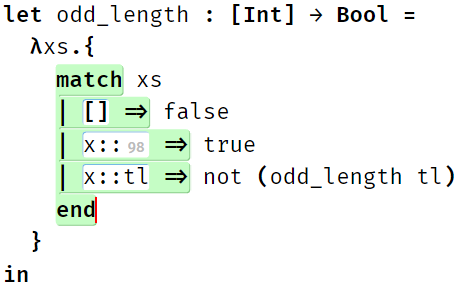
\includegraphics[scale=0.45,valign=t]{imgs/exhaustive.png}
%	}
%	\caption{Exhaustiveness Checking with Pattern Holes}
%	\label{fig:exhaustiveness}
%\end{figure}
%
%\subsection{Redundancy Checking with Pattern Holes}
%
%\begin{figure}
%	\centering
%	\subcaptionbox{Necessarily Irredundant (first two patterns) + Indeterminately Irredundant (third pattern)\label{fig:may-redundant}}{
%		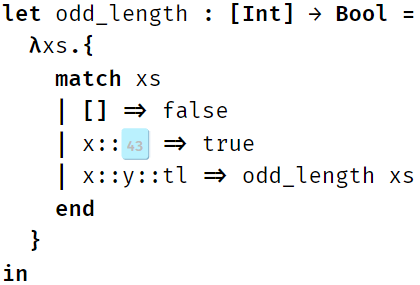
\includegraphics[scale=0.5,valign=t]{imgs/maybe_redundant.png}%
%		\vphantom{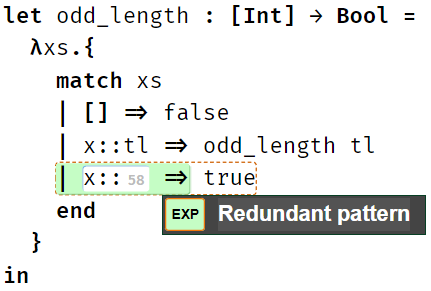
\includegraphics[scale=0.5,valign=t]{imgs/redundant.png}}
%	} 
%	\hfil
%	\subcaptionbox{Necessarily Redundant (third pattern) \label{fig:must-redundant}}{
%		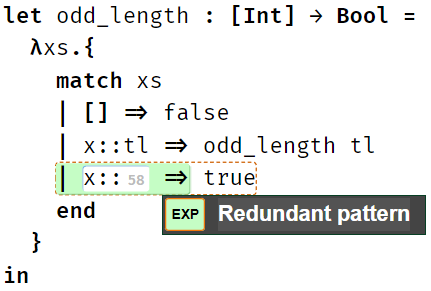
\includegraphics[scale=0.5,valign=t]{imgs/redundant.png}
%	}%
%	\caption{Redundancy Checking with Pattern Holes}
%	\label{fig:redundancy}
%\end{figure}
%
%\subsection{Live Evaluation with Pattern Holes}
%
%\begin{figure}
%	\centering
%	\subcaptionbox{Pattern matching with expression holes\label{fig:exp-hole}}{
%		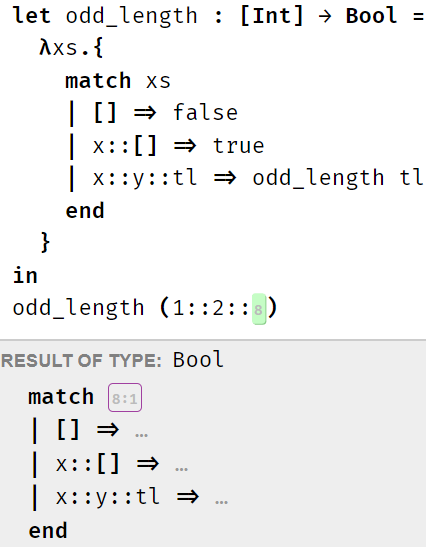
\includegraphics[scale=0.47,valign=t]{imgs/pat_match_exp_holes.png}
%		\vphantom{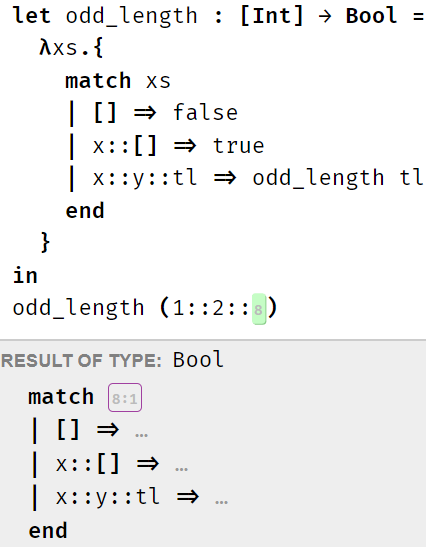
\includegraphics[scale=0.47,valign=t]{imgs/pat_match_exp_holes.png}}
%	}
%	\hfil
%	\subcaptionbox{Pattern matching with pattern holes\label{fig:pat-hole}}{
%		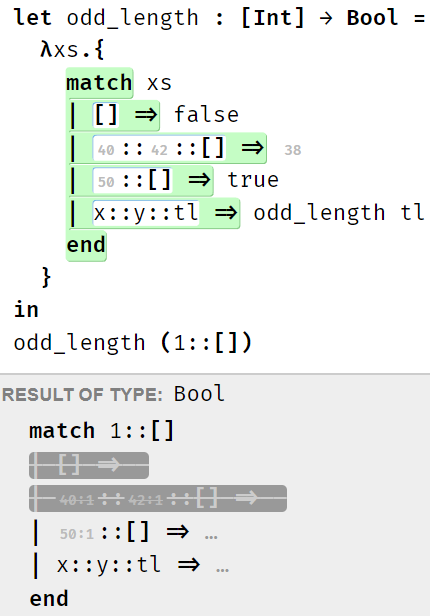
\includegraphics[scale=0.47,valign=t]{imgs/pat_match_pat_holes.png}
%	}
%	\caption{Live Evaluation with Expression and Pattern Holes}
%	\label{fig:evaluation-ex}
%\end{figure}

